% !TeX root = ../libro.tex
% !TeX encoding = utf8

\chapter{Resultados principales}

\section{Enunciados}
	\begin{teora}
		Toda variedad topológica 2-dimensional tiene una estructura diferenciable.
	\end{teora}

	\begin{teorb}
		Todo homeomorfismo entre variedades diferenciables 2-dimensionales es isotópico a un difeomorfismo.
	\end{teorb}
	
	Suponiendo ciertos los teoremas anteriores, es directa la obtención del siguiente resultado, ya que por A tenemos que toda variedad topológica 2-dimensional tiene una estructura diferenciable y por B sabemos que es única salvo difeomorfismos:
	
	\begin{corolario} (Teorema clásico de Munkres)
		Toda variedad topológica 2-dimensional tiene una única estructura diferenciable salvo difeomorfismos.
	\end{corolario}

\section{Demostración del Teorema A}

	\begin{teora}
		Toda variedad topológica tiene una estructura diferenciable.
	\end{teora}
	\begin{proof}[Demostración]
		Sea S una variedad topológica, podemos coger un atlas $\{h_i | 1\leq i < N\}$ con $N \in \N$ si es finito o $N = \infty$ si no lo es. Vamos a construir por inducción una estuctura diferenciable en el conjunto $U_n = \cup_{i\leq n}h_i(\R^2)$ para cada $n < N$, que por tratarse de sistemas coordenados de un atlas su límite debe de ser S, probando así el resultado. Cabe destacar que cada $U_n$ contiene a todos los anteriores. \\
		\\ La inducción empieza tomando una carta cualquiera del sistema, $U_1=h_1(\R^2)$ por ejemplo. Si se considera la variedad $U_1$ con el atlas $\{h_1\}$ entonces $h_1$ es diferenciable para ésta de forma trivial (se compone con la inversa y queda la identidad en $\R^2$).\\
		\\ Una vez arrancada la inducción, suponiendo cierto para el paso $n-1$ vamos a extender la diferenciabilidad de $U_{n-1}$ a $U_n$. Sea la carta $h_n$, tomamos entonces $W=h_n^{-1}(U_{n-1})=h_n^{-1}(U_{n-1}\cap h_n(\R^2))$, que es un abierto de $\R^2$ por ser $h_n$ continua. \\
		\\ Tenemos $W\subset \R^2$ abierto, por el \textbf{Hecho 1} sabemos que existe una triangulación geométrica suya y al ir acercándose a la frontera topológica los triángulos convergen a puntos. Queremos aplicar el ``Teorema de alisamiento de asas'' en los vértices de los triángulos, seguidamente en los lados y finalmente en el interior de cada triángulo (aplicar los 3 apartados del teorema de forma consecutiva), pero para ello es necesario partir de un embebimiento de $\R^2$:
		\begin{enumerate}
			\item Para todos y cada uno de los vértices de la triangulación elegimos una bola $B(p, \epsilon_p) \subset W$ cuyos cierres topológicos en $\R^2$ no se corten mutuamente. $B(p,\varepsilon _p)$ es abierto y queremos obtener $\widehat{h}$ diferenciable entorno a $p$. \\
			\newpage
			\begin{figure}[h]
  				\centering
  				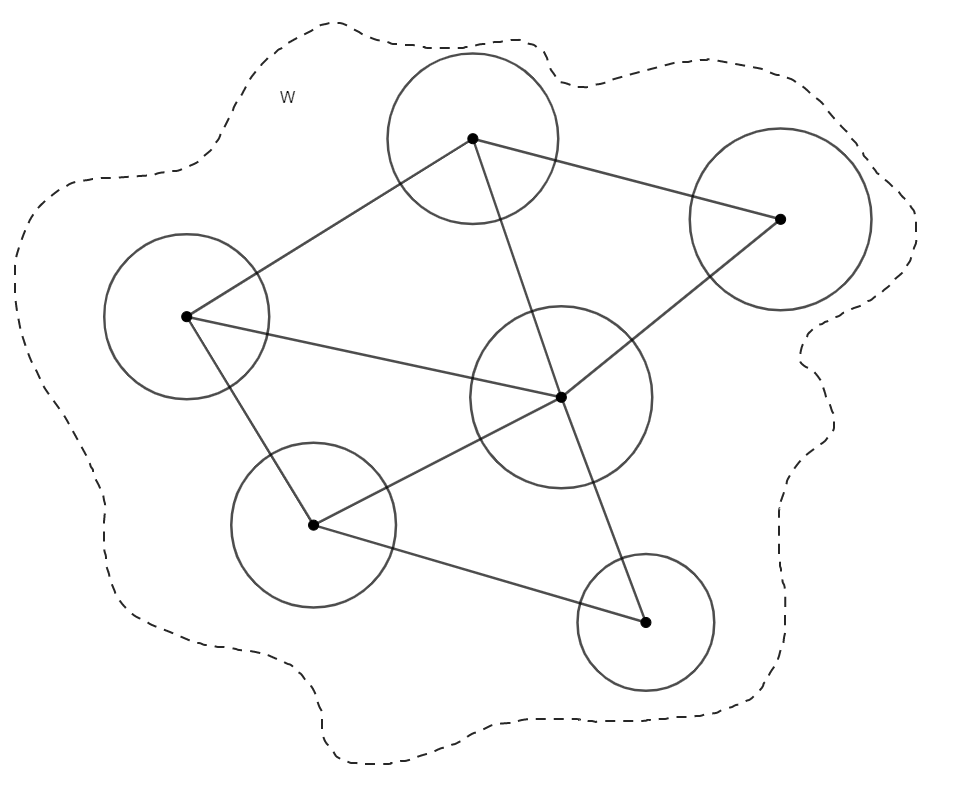
\includegraphics[width=0.5\textwidth]{triangulacion_bolas}
  				\caption{$B(p, \epsilon_p)$ para cada vértice.}
  				\label{fig:triangulacion_bolas}
			\end{figure}
			Podemos aplicar el Corolario del apartado 1 del Teorema de Alisamiento de Asas ya que cumplimos todas las hipótesis necesarias. Así obtenemos una $\widehat{h}$ isotópica a $h$, que es diferenciable en $O_p$ entorno abierto de $p$ y además queda fija fuera de otro entorno un poco mayor $O_p'\supset O_p$, con $O'_p\subset B(p, \epsilon_p) $.\\
			\\ De manera acumulativa, este procedimiento se puede realizar simultáneamente en todos los vértices $p$ en la triangulación de $W$. Esto prueba que $h_n: W \rightarrow U_{n-1}$ es isotópica a un homeomorfismo $\widehat{h}_n: W \rightarrow U_{n-1}$ que es diferenciable, como aplicación sobre la superficie diferenciable $U_{n-1}$, en un entorno $O_p \subset W$ alrededor de cada vértice $p$ de la triangulación de $W$. Además la isotopía coincide con $h_n$ fuera de entornos $O'_p \subset W$ mayores que $O_p$ para cada $p$, disjuntos $2$ a $2$.\\
			\begin{figure}[h]
  				\centering
  				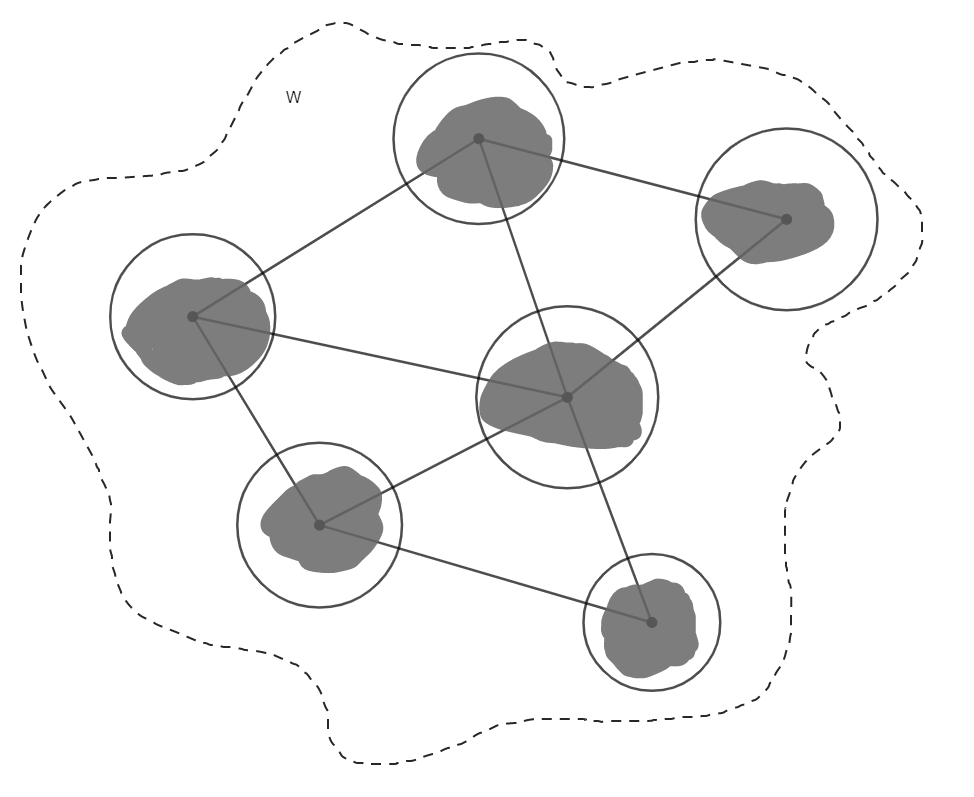
\includegraphics[width=0.5\textwidth]{triangulacion_bolas_suavizado}
  				\caption{$O_p$ para cada vértice.}
  				\label{fig:triangulacion_bolas_suavizado}
			\end{figure}

			\item Tenemos por el paso anterior un $h_n: \R^2 \rightarrow h_n(\R^2)$ isotópico al original en las condiciones explicadas, y que es diferenciable como aplicación $W \rightarrow U_{n-1}$ entorno a los vértices de la triangulación de $W$. Queremos utilizar el apartado $2$ del Teorema de Alisamiento de Asas para generar otra isotopía que nos lleve $h_n$ a otro homeomorfismo (al que le daremos el mismo nombre) cuya restricción a $W \rightarrow U_{n-1}$ sea diferenciable además entorno a los lados de la triangulación anterior, coincidiendo con el $h_n$ original fuera de un entorno del $1$-esqueleto de esa triangulación.\\
			\\ Para ello, consideramos para cada lado $l$ de la triangulación de $W$ un subconjunto $R_l$ (rectángulo) dentro de $W$ que sea difeomorfo a $D^1 \times \R$, cumpliendo:
				\begin{enumerate}
					\item $R_l$ corta a $l$ en un segmento compacto y es disjunto con cualquier otro lado de la triangulación de $W$. En particular, $R_l$ no contiene ningún vértice de la triangulación de $W$.
					\item Si $p_1$ y $p_2$ son los vértices extremos de $l$, una componente del borde de $R_l$ está contenida en $O_{p_1}$ y la otra en $O_{p_2}$, es decir, $h_n$ es diferenciable en 2 componentes de $\partial R_l$.
					\item Los cierres de los rectángulos $R_l$ en $\R^2$ son disjuntos $2$ a $2$ y están contenidos en $W$.
				\end{enumerate}
			\begin{figure}[h]
  				\centering
  				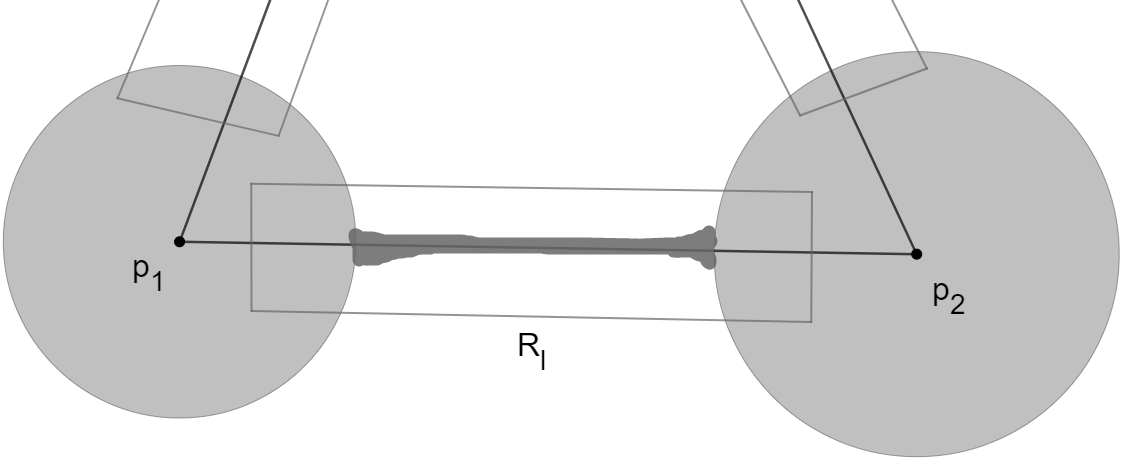
\includegraphics[width=0.5\textwidth]{triangulacion_rectangulos_suavizado}
  				\caption{Entorno de $l$ donde $h_n$ es diferenciable.}
  				\label{fig:triangulacion_rectangulos_suavizado}
			\end{figure}

			Ahora es evidente como en el apartado $2$ del Teorema de Alisamiento de Asas nos produce la isotopía deseada realizando el trabajo simultáneamente en todos los rectángulos $R_l$, generando el nuevo $h_n:\R^2 \rightarrow h_n(\R^2)$ deseado.
			\begin{figure}[h]
  				\centering
  				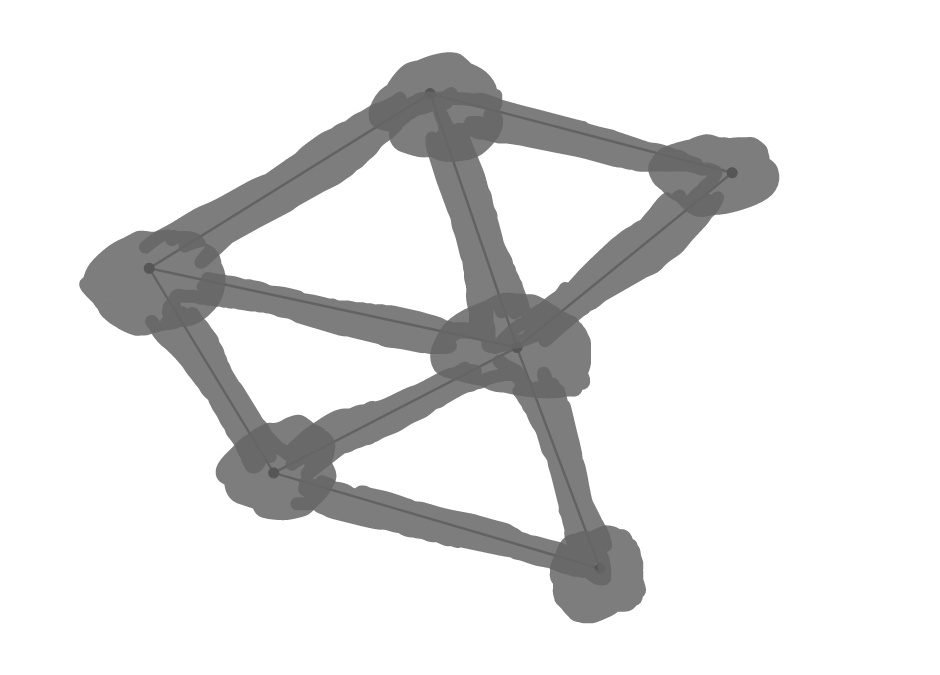
\includegraphics[width=0.45\textwidth]{triangulacion_aristas}
  				\caption{Entorno del $1$-esqueleto donde $h_n$ es diferenciable.}
  				\label{fig:triangulacion_aristas}
			\end{figure}

			\item El tercer paso es similar a los anteriores, pero ahora usando el apartado $3$ del Teorema de Alisamiento de Asas. Lo que hacemos en considerar para cada triángulo $T$ de la triangulación de $W$ un dominio de Jordan $D_T$ satisfaciendo:
			\begin{enumerate}
				\item $D_T \subset \mathring{T}$.
				\item $h_n:W \rightarrow U_{n-1}$ es diferenciable sobre $T-\mathring{D_T}$.
				\item Los $D_T$ son disjuntos dos a dos.
			\end{enumerate}
			
			Aplicando el Teorema de Carathéodory obtenemos que es difeomorfo a la bola unidad y por tanto podemos proceder de manera similar a los apartados anteriores. \\
			\\ A continuación producimos otra isotopía que nos lleve el $h_n$ generado en el apartado $2$ a otro homeomorfismo (al que daremos el mismo nombre) cuya restricción $W \rightarrow U_{n-1}$ sea diferenciable sobre $D_T$, coincidiendo en cada instante con la $h_n$ anterior en un entorno de $\partial D_T$ y de hecho fuera de $D_T$, para cada triángulo $T$. Esto concluiría la prueba. \\
			\\ Para probar la existencia de $D_T$ vamos a definir la curva de Jordan cuyo interior es de forma trivial un dominio de Jordan, que será dicho $D_T$. La curva debe ser diferenciable, cerrada y simple, que es la caracterización de una curva de Jordan. Reducimos el problema a buscar dicha curva para el entorno tubular de un triángulo equilátero, ya que es difeomorfo al de un triángulo cualquiera. Podemos simplificarlo más aportando únicamente una curva no cerrada cuyos extremos se puedan pegar consecutivamente, siendo infinitamente derivable en los puntos donde se unen.\\
			\\ Haciendo uso de una función meseta $f$ que vale $0$ en $\mathbb{R}^-$ y $1$ a partir de $\epsilon > 0$, si tomamos $g(x)=tg(\frac{\pi}{3})xf(x)$ en el intervalo $[-1,\epsilon]$, tenemos que $g(-1)=0$ y $g(\epsilon)=tg(\frac{\pi}{3})\epsilon$  al igual que sus derivadas, por lo que si vamos alternando $g(x)$ y $g(-x)$ mediante rotaciones y traslaciones, tendremos una curva $\alpha$ diferenciable (suavización del triángulo equilátero). \\
			%\newpage
			\begin{figure}[h]
  				\centering
  				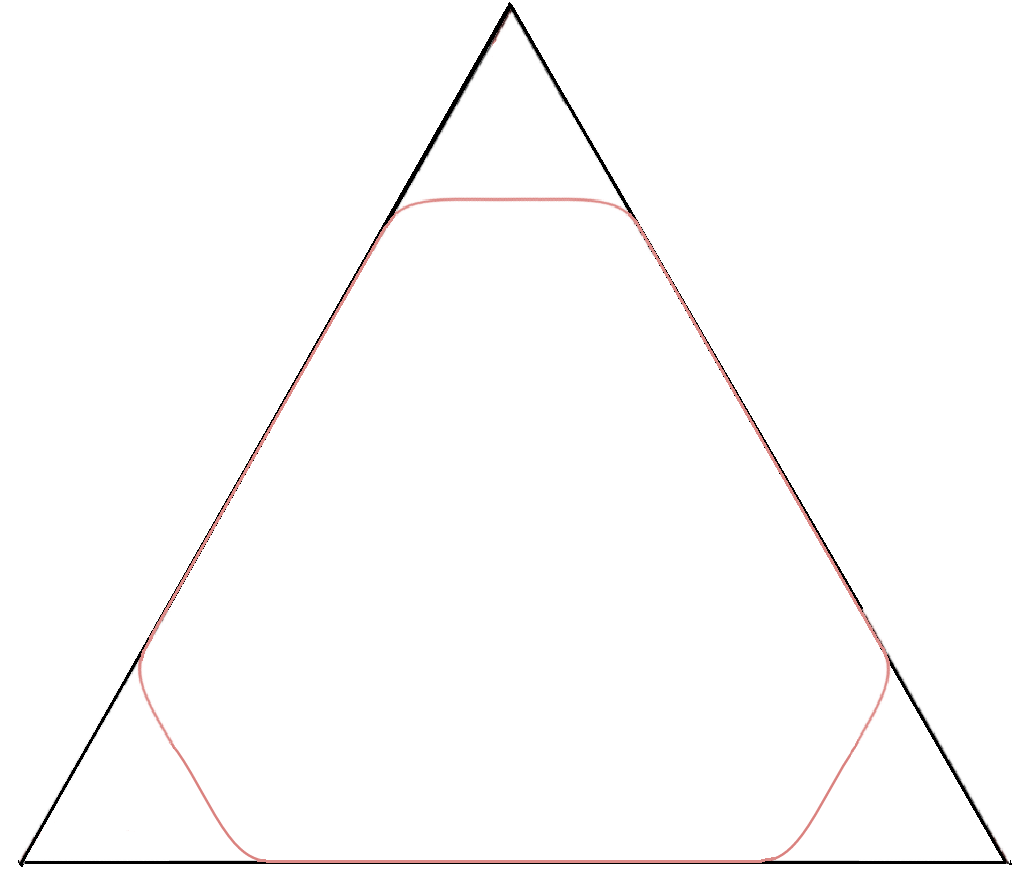
\includegraphics[width=0.5\textwidth]{triangulo_suavizado}
  				\caption{Curva de Jordan cercana al triángulo}
  				\label{fig:triangulo_suavizado}
			\end{figure}
			\\ Se puede observar que es válido $\forall \epsilon > 0$ y que al hacer tender $\epsilon$ a $0$, la curva será el propio triángulo equilátero. Es por ello que podemos tomar el $\epsilon$ lo suficientemente pequeño como para que la curva $\alpha$ quepa en el entorno tubular y siga siendo una curva de Jordan. Como exigimos que $D_T \subset \mathring{T}$ podemos aplicar a la curva un factor de escala para así no contener ningún punto del borde del triángulo $T$. Además, de forma evidente obtenemos que los dominos $D_T$ son disjuntos $2$ a $2$.
		\end{enumerate}

		Todas las isotopías de los pasos anteriores coinciden por extensión continua con el homeomorfismo $h_n:\R^2 \rightarrow h_n(\R^2)$ original en la frontera de $W$ en $\R^2$ por construcción, ya que el diámetro de los triángulos en $W$ tiende a $0$ al acercarnos a la frontera. Por tanto pueden ser extendidas como isotopías de $\R^2 \rightarrow h(\R^2)$ coincidentes con $h_n$ en $\R^2 - W$. \\
		\\ Como conclusión, el homeomorfismo $h_n:\R^2 \rightarrow h_n(\R^2)$ resultante es compatible con la estructura diferenciable en $U_{n-1}$ y junto con $h_1$, $\ldots$, $h_{n-1}$, nos define una estructura diferenciable sobre $U_n$. Esto cierra la inducción y prueba el teorema. \\
	\end{proof}

\section{Demostración del Teorema B}
	\begin{teorb}
		Todo homeomorfismo entre variedades diferenciables 2-dimensionales es isotópico a un difeomorfismo.
	\end{teorb}
	\begin{proof}[Demostración]
		Sea $f:S\to S’$ un homeomorfismo entre superficies diferenciables. Por el Hecho $2.2$ (ver su demostración) podemos encontrar una triangulación clásica en el sentido de Radó de $S$ que también sea diferenciable. Eso significa que las $2$-celdas son embebimientos diferenciables de triángulos geométricos en $\R^2$ en $S$, las  $1$-celdas embebimientos diferenciables de segmentos de $\R^2$ en $S$, y las $0$-celdas (vértices de la triangulación) puntos en $S$. La prueba sigue las mismas ideas del Teorema A.
	\begin{enumerate}
		\item Para cada uno de los vértices $p$ de la triangulación se considera una carta diferenciable $\varphi_p : \overline{D}\to \overline{B}_p\subset S$, $\varphi_p(D)=B_p$, $\varphi_p((0,0))=p$, donde como siempre $D$ es el disco unidad abierto y $ \overline{D}$ el cerrado en $\R^2$. Haremos la elección de cartas de forma que los discos topológicos $\{\overline{B}_p \colon p$ vértice de la triangulación$\}$ sean disjuntos dos a dos. Para cada vértice $p$ llamaremos $g_p=f\circ \varphi_p:D\to f(B_p)\subset S’$, y procediendo como en el Apartado $1$ de la demostración del Teorema A, encontraremos un homeomorfismo $\hat g_p:D\to f(B_p)$ isotópico a  $g_p$, diferenciable en un entorno $O_p$ de $(0,0)$, y que coincida con $g_p$ fuera de un entorno compacto $O’_p$  de $(0,0)$ en $D$ conteniendo a $O_p$. En particular el homeomorfismo $\hat \varphi_p=\hat g_p\circ \varphi_p^{-1}:B_p\to f(B_p)$ es isotópico a  $f|_{B_p}$, diferenciable en un entorno de $p$, y que coincide con $f$ fuera de un entorno compacto de $p$ en $B_p$. Todas estas últimas isotopías se pegan de forma natural, extendidas como $f$ fuera de las bolas $B_p$, para construir una isotopía entre $f$ y un homeomorfismo $\hat f\colon S\to S’$ que es diferenciable en el abierto  $O=\cup_p \varphi_p(O_p)$, y coincide con $f$ fuera de  $O’=\cup_p \varphi_p(O’_p)$.

		\item Al homomorfismo $\hat f$ generado en el apartado anterior, por comodidad en la notación, le seguiremos llamando $f$. Para cada uno de los lados $l$ de la triangulación se considera una carta diferenciable $\varphi_l\colon [-1,1]^2\to \overline{R}_l\subset S$, $\varphi_l([-1,1]\times ]-1,1[)=R_l$, $\varphi_l([-1,1] \times 0)=l_0$, donde $l_0$ es un subsegmento de $l$ no conteniendo sus extremos. Haremos la elección de cartas de forma que los discos topológicos $\{\overline{R}_l\colon l$ lado de la triangulación$\}$ sean disjuntos dos a dos y además $\varphi_l(D^1 \times [-1,1])\subset O$, donde $D^1=\{-1, 1\}$. Para cada lado $l$ llamaremos $g_l=f\circ \varphi_l:[-1,1]\times ]-1,1[\to f(R_l)\subset S’$, y procediendo como en el Apartado $2$ de la demostración del Teorema A, encontraremos un homeomorfismo $\hat g_l:[-1,1]\times ]-1,1[\to f(R_l)$ isotópico a  $g_l$, diferenciable en un entorno $U_l$ de $[-1,1] \times 0$, y que coincida con $g_l$ en $U’_l$, donde $U’_l$ ahora es la unión de un entorno de $D^1 \times ]-1,1[$ en $[-1,1]\times ]-1,1[$  y el complemento de un entorno compacto de $[-1,1] \times 0$ en $[-1,1]\times ]-1,1[$ conteniendo a $U_l$. En particular el homeomorfismo $\hat \varphi_l=\hat g_l\circ \varphi_l^{-1}:R_l\to f(R_l)$ es isotópico a  $f|_{R_l}$, diferenciable en un entorno de $l_0$, y  coincide con $f$ en un entorno de $\partial R_l$ y fuera de un entorno compacto de $l_0$ en $R_l$. Todas estas últimas isotopías se pegan de forma natural, extendidas como $f$ fuera de los rectángulos topológicos $R_l$, para construir una isotopía entre $f$ y un homeomorfismo $\hat f\colon S\to S’$ que es diferenciable en un entorno $U$ del $1$-esqueleto de la triangulación y coincide con $f$ fuera de un entorno cerrado $\overline{U}’$ de ese $1$-esqueleto conteniendo a $\overline U$ en su interior $U’$.

		\item Al homomorfismo $\hat f$ generado en el apartado anterior, por comodidad en la notación, le seguiremos llamando $f$.  En éste último paso para cada uno de los triángulos $T$ de la triangulación tomaremos una carta diferenciable $\varphi_T\colon \Delta \to T\subset S$, donde $\Delta$ representa la envolvente convexa en $\R^2$ de los puntos $(-1,0), (1,0), (0,1)$. Consideraremos también un disco abierto $D_T \subset \Delta$ con borde diferenciable de forma que $\varphi_T(\Delta\setminus D_T)\subset U$, y llamaremos $g_T=f\circ \varphi_T:\Delta \to f(T)\subset S’$. Procediendo como en el Apartado 3 de la demostración del Teorema A, encontraremos un difeomorfismo $\hat g_T:\Delta\to f(T)$ isotópico a  $g_T$ y que coincida con $g_T$ en un entorno de $\partial \Delta$. En particular el difeomorfismo $\hat \varphi_T=\hat g_T\circ \varphi_T^{-1}:T\to f(R_l)$ es isotópico a  $f|_{T}$ y  coincide con $f$ en un entorno de $\partial T$. Todas estas últimas isotopías se pegan de forma natural para construir una isotopía entre $f$ y un difeomorfismo global $\hat f\colon S\to S’$, completando la prueba.
		\end{enumerate}
	\end{proof}
\endinput
%------------------------------------------------------------------------------------
% FIN DEL CAPÍTULO. 
%------------------------------------------------------------------------------------
